% $Author: stef $
% $Date: 2008-04-04 17:14:31 +0200 (Fri, 04 Apr 2008) $
% $Revision: 318 $
%=================================================================
\ifx\wholebook\relax\else
% --------------------------------------------
% Lulu:
    \documentclass[a4paper,10pt,twoside]{book}
    \usepackage[
        papersize={6in,9in},
        hmargin={.75in,.75in},
        vmargin={.75in,1in},
        ignoreheadfoot
    ]{geometry}
    \input{../common.tex}
    \pagestyle{headings}
    \setboolean{lulu}{true}
% --------------------------------------------
% A4:
%   \documentclass[a4paper,11pt,twoside]{book}
%   \input{../common.tex}
%   \usepackage{a4wide}
% --------------------------------------------
    \graphicspath{{figures/} {../figures/}}
    \begin{document}
%   \renewcommand{\nnbb}[2]{} % Disable editorial comments
    \sloppy
\fi
\chapter{Directions et Angles}\label{cha:turning}

\noindent\hrule
\hfil 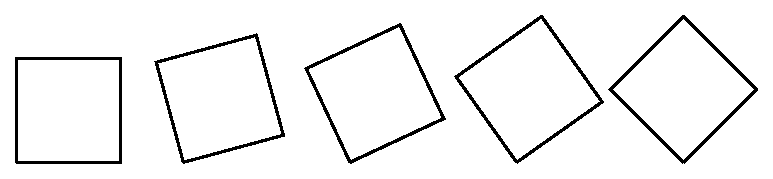
\includegraphics[width=0.9\linewidth]{ChTurntitlePicture}\hfil
\vspace{0.2cm}
\noindent\hrule\vspace{1.5cm}


A pr\'esent, vous devriez \^etre fatigu\'e de dessiner des figures que dans des directions fixes. 
Dans ce chapitre vous apprendrez comment changer la direction dans laquelle le robot pointe, 
comment permettre au robot de pointer dans n'importe quelles directions, tourner \`a n'importe 
quels angles relatifs \`a sa position courante, et par cons\'equent dessiner des lignes dans n'importe 
quelles directions. Si vous comprenez clairement ce qu'est un angle et comment mesure-t-on les angles en degr\'es, 
vous devriez sauter la section "L'Angle Droit des Choses" et poursuivre ensuite aux exemples et exercices de la section "Simple Dessins".
Je commencerai par pr\'esenter les messages \'el\'ementaires pour changer de directions que comprend le robot. 
Je vais cachez les robots des illustrations en utilisant le message \ct{beInvisible} pour rendre les images plus claires.

\newpage

\section{Droite ou Gauche?}

Dans le pr\'ec\'edent chapitre, vous avez appris qu'un robot peut \^etre orient\'e dans diff\'erentes directions 
en utilisant les messages \ct{east}, \ct{north}, \ct{northEast}, \ct{northWest}, \ct{south},
\ct{southEast}, \ct{southWest}, and \ct{west}. 
Toutefois, avec ces messages vous ne pouvez pas changer la direction de votre robot par un angle arbitraire, 
tel que 15 degr\'es. En plus, vous ne pouvez pas tourner un robot, en disant, un quart de tour par rapport \`a 
sa position courante.

Pour faire tourner un robot d'un angle donn\'e vous devez utilisez les deux instructions \ct{turnLeft:} et 
\ct{turnRight:}, qui disent au robot de tourner \`a gauche ou \`a droite. Les deux points \`a la fin de chaque 
nom de m\'ethode indique que ces deux m\'ethodes attendent un argument. Cet argument est l'angle de rotation 
que devra effectuer le robot par rapport \`a sa position courante. C'est-\`a-dire l'argument est la diff\'erence 
entre la direction du robot avant le message envoy\'e et sa direction apr\`es que le message lui a \'et\'e envoy\'e. 
Cet angle est donn\'e en degr\'es. Par exemple l'expression \ct{pica turnLeft: 15} 
demande \`a pica de tourner \`a gauche de quinze degr\'es par rapport \`a sa position courante, et \ct{pica turnRight: 30} 
demande \`a pica de tourner de trente degr\'es \`a droite par rapport \`a sa position courante. La Figure ~\ref{fig:turnLeftBoth} 
illustre l'effet du message \ct{turnLeft:} et \ct{turnRight:}, en premier quand un robot pointe \`a l'est, et en second quand un robot pointe dans une autre direction.

\begin{figure}
\begin{center}\includegraphics[width=12cm]{turnLeftBoth}
\caption{A gauche : un robot  face \`a l'est tourne \`a gauche ou \`a droite de 30 degr\'es. A droite : un robot face \`a n'importe 
quelle autre direction tourne \`a gauche ou \`a droite de 30 degr\'es \label{fig:turnLeftBoth}}
\end{center}
\end{figure}

Lorsque vous vous exercez \`a faire tourner le robot de diff\'erents angles, 
gardez en m\'emoire que quand un nouveau robot est cr\'e\'e, il pointe toujours \`a l'est, c'est-\`a-dire, \`a droite de l'\'ecran.




\begin{exonofig}{Des Scripts Myst\'erieux}
Les Scripts ~\ref{scr:myster1} et \ref{scr:myster2} pr\'esentent des probl\`emes dans lesquels vous supposez que les robots cr\'e\'es les r\'ealiseront. Apr\`es avoir \'etudi\'e ces deux scripts, entrainez vous avec eux en changeant les valeurs des angles, par exemple pour d\'eterminer que l'angle de rotation que doit effectuer le robot est un quart de cercle, un demi-cercle, ou un cercle entier. Si vous avez besoin de revoir les notions d'angle, lisez la section "L'Angle Droit des Choses" avant de continuer.
\end{exonofig}

\begin{script}[myster1]{Que fait pica ? (Probl\`eme 1)}
	| pica | 
	pica := Bot new. 
	pica go: 100. 
	pica turnLeft: 45. 
	pica go: 50. 
	pica turnLeft: 45. 
	pica go: 100 
\end{script}

\begin{script}[myster2]{Que fait pica ? (Probl\`eme 2)}
	| pica | 
	pica := Bot new. 
	pica go: 100. 
	pica turnRight: 60. 
	pica go: 100. 
	pica turnLeft: 60. 
	pica go: 100 
\end{script}


\section{Une convention directionnelle}

En math\'ematique, une convention g\'en\'erale est que la rotation \`a angle n\'egative est interpr\'et\'ee dans le sens des aiguilles 
d'une montre, tandis que la rotation avec un angle positif est interpr\'et\'ee dans le sens inverse des aiguilles d'une montre. 
Vous pouvez utiliser cette convention math\'ematique en se servant du message \ct{turn:}. D'où le message 
\ct{turnLeft: aNumber} est \'equivalent au message \ct{turn: aNumber}, wtandis que le message \ct{turnRight: aNumber} est \'equivalent \`a \ct{turn: -aNumber}, où \ct{-aNumber} est l'inverse de \ct{aNumber}. 
relation est repr\'esent\'e par la Figure~\ref{fig:turnLeftWithMathematicalEq}. 


\begin{figure}
\begin{center}\includegraphics[width=8cm]{turnLeftWithMathematicalEq}
\caption{Rotation d'un angle de 30 degr\'es en partant de la direction est. \label{fig:turnLeftWithMathematicalEq}}
\end{center}
\end{figure}





\section{Orientation Relative contre Orientation Absolue}
Vous devez maintenant \^etre confiant quand au fait de pouvoir demander au robot d'executer n'importe quels dessins 
compos\'es de lignes droites. Avant d'aller plus loin, il faut \^etre certain que vous compreniez la diff\'erence entre 
l'orientation d'un robot absolue en utiilisant les m\'ethodes \ct{north}, \ct{south}, \ct{southEast}, \ct{east}, etc., et en utilisant 
les m\'ethodes \ct{turn:}, \ct{turnLeft:}, et \ct{turnRight:} pour orienter le robot relatif  \`a son orientation courant. 
Les Exercices \ref{xp:relsq}, \ref{xp:titledsquare}, et \ref{xp:brsquare} vous aiderons \`a solidifier votre compr\'ehension sur cette diff\'erence.



\begin{exofigwithsize}[0.7]{\includegraphics[width=2.5cm]{ChTurnfirstSquare}}{Un Carr\'e Relatif}\label{xp:relsq}
Ecrivez un script qui dessine un carr\'e en utilisant la m\'ethode \ct{turnLeft:} ou \ct{turnRight:}. 
\end{exofigwithsize}


\begin{exonofigtitle}{Un Carr\'e Inclin\'e}\label{xp:titledsquare}
Modifiez votre script de l'Exercice ~\ref{xp:relsq} en ajoutant la ligne \ct{pica turnLeft: 33.} avant la premi\`ere ligne contenant le message \ct{go: 100}. Vous obtiendrez encore un carr\'e, mais il sera inclin\'e de 33 degr\'es par rapport au carr\'e pr\'ec\'edent. 
\end{exonofigtitle}




\begin{exonofigtitle}{Un carr\'e cass\'e}\label{xp:brsquare}
Finalement, ex\'ecutez le Script ~\ref{scr:brsquare}, qui tente de dessiner un carr\'e inclin\'e en utilisant les m\'ethodes \ct{north}, \ct{south}, \ct{east}, et \ct{west} que nous avons vues dans le chapitre pr\'ec\'edent. 
\end{exonofigtitle}


\begin{scriptfigwithsize}[0.4]{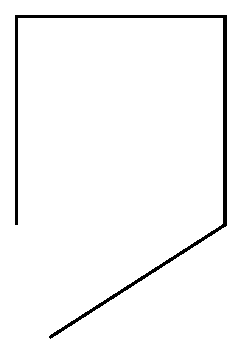
\includegraphics[width=3cm]{ChTurnbadSquare}}{Un Carr\'e Cass\'e}\label{scr:brsquare}
	| pica | 
	pica := Bot new. 
	pica north. 
	pica go: 100. 
	pica east. 
	pica go: 100. 
	pica south. 
	pica go: 100. 
	pica north. 
	pica go: 50. 
	pica west. 
	pica go: 100
\end{scriptfigwithsize}

DObtenez vous encore un carr\'e ? Non ! le premier cot\'e dessin\'e par le robot est de travers, tandis que les autres cot\'es 
sont soit horizontaux soit verticaux. Le script que vous avez \'ecrit pour l'Exercice ~\ref{xp:brsquare} avec le 
Script~\ref{scr:brsquare} d\'emontre la diff\'erence cruciale entre les changements \emph{relative} et \emph{absolute}
 dans des directions : 

\begin{itemize}
\item Les m\'ethodes \ct{north}, \ct{south}, \ct{east}, et \ct{west} changent de direction d'une mani\`ere absolue. 
La direction dans laquelle le robot pointera \emph{ne d\'epend pas} de la direction actuelle 
vers laquelle le robot pointe.
\item  Les m\'ethodes \ct{turnLeft:} et \ct{turnRight:} cchangent de direction d'une mani\`ere relative. 
La direction dans laquelle le robot pointera \emph{depend} de sa direction actuelle. 
\end{itemize}

La Figure~\ref{fig:roserelative} montre l'\'equivalence entre les mouvements relatifs commençant avec un robot 
pointant vers l'est et les mouvements absolus. Comme vous le savez cette \'equivalence est valide seulement si 
le robot pointe vers l'est et pas dans une autre direction. A propos, notons que la rotation d'un robot \`a 
180 degr\'es pointe dans la direction oppos\'ee ; cette combine est souvent utilis\'ee dans les scripts.


\begin{figure}[h]
\begin{center}\includegraphics[width=8cm]{roseDesVentsRelatifToo}
\caption{Comparaison d'une orientation absolue et relative partant de la direction est.\label{fig:roserelative}}
\end{center}
\end{figure}

\section{L'Angle Droit des Choses}

Comme vous le savez maintenant, un nouveau robot cr\'e\'e pointe vers l'est, vers le côt\'e droit de l'\'ecran. 
Si vous demandez \`a ce robot de tourner \`a gauche de 90 degr\'es, il aura la t\^ete vers le nord. Si \`a la place, 
nous lui demandons de tourner \`a droite de 90 degr\'es, il pointera vers le sud. Le script 4-4 illustre le 
r\'esultat d'un tour \`a gauche de 45 degr\'es. Pour vous aider \`a suivre le script, la figure accompagnante montre 
la position de d\'epart du robot.

\begin{scriptfigwithsize}[0.5]{\includegraphics[width=5cm]{ChTurnAngleSearchAnnotated}}{Mouvement par les angles (1)}\label{xp:angle1}
	| pica | 
	pica := Bot new. 
	pica west. 
	pica go: 100. 
	pica east. 
	pica turnLeft: 45. 
	pica go: 100.
\end{scriptfigwithsize}



La premi\`ere partie du Script~\ref{xp:angle1}, au dessus de la ligne pica east, dessine une ligne horizontale, 
qui agira comme une ligne de r\'ef\'erence pour indiquer la direction vers l'est. La derni\`ere partie dessine une 
ligne dans la direction de 45 degr\'es \`a gauche de la direction est. Vous pouvez faire varier les valeur des 
angles pour voir quelles sorte d'angle repr\'esente les autres valeurs de degr\'es. Essayez les valeurs 
60, 120, 180, 240, 360 et 420. En particulier, notez qu'un tour de 180 degr\'es fait tourner le robot dans la 
direction oppos\'ee vers laquelle il pointe.

Voyez vous une diff\'erence entre les arguments 60 et 420 degr\'es ? Ils repr\'esentent le m\^eme angle ! 
Deux valeurs qui ont une diff\'erence de 360 degr\'es ou un multiple de celui-ci sont \'equivalent car 360 degr\'es 
repr\'esente un cercle complet. essayez un angle d'une valeur de 1860 (1860=60+360*5). Vous obtenez le m\^eme 
r\'esultat qu'avec un angle de 60 degr\'es et 420 degr\'es. Gardons en m\'emoire la relation avec les angles, que 
l'orientation d'un robot ne change pas en ajoutant un ou plusieurs tours \`a l'orientation.

Maintenant amusons nous un peu avec la m\'ethode \ct{turnRight:}. Le Script 4-5 dessine les aiguilles des heures 
et des minutes d'une horloge avec une ligne de r\'ef\'erence. Il utilise deux robots, que vous pouvez utiliser pour 
examiner la correspondance entre le tour \`a gauche et le tour \`a droite. J'ai ajout\'e des commentaires mis entre 
guillemets et ai employ\'e une vari\'et\'e de police pour vous aider \`a identifier les diff\'erentes parties du script. 
Notons que vous n'avez pas \`a taper ces commentaires, du fait qu'il ne sont pas ex\'ecut\'es. 


\begin{scriptfigwithsize}[0.4]{\includegraphics[width=7cm]{twoAnglesAnnotated}}{Mouvement par les  angles (2)}\label{xp:angle2}
	| pica daly | 
	pica := Bot new. 
	pica jump: 200. 
	"drawing the reference line" 
	pica turnLeft: 180. 
	pica go: 200. 
	pica turnLeft: 180. 
	pica color: Color blue. 
	pica turnLeft: 45.       
	"drawing the minute hand" 
	pica go: 150. 
	daly := Bot new. 
	daly color: Color red. 
	\textbf{daly turnRight: 45.}  
	"drawing the hour hand" 
	\textbf{daly go: 100.} 
\end{scriptfigwithsize}


Dans le Script~\ref{xp:angle2}, le code en italique dessine la ligne de r\'ef\'erence—c'est la ligne 
repr\'esentant la direction du robot avant que la m\'ethode pour tourner ne soit ex\'ecut\'e—utilisant un tour de 180 degr\'es 
pour tourner et pointer dans la direction oppos\'ee. La ligne de r\'ef\'erence est \'egalement la plus longue ligne trac\'ee. La ligne 
de r\'ef\'erence sera encore visible si les lignes dessin\'ees par les robots tombent au dessus de celle-ci. Le texte 
dans la police roman normale suivant l'italique est le code qui dessine l'aiguille des minutes 
(en utilisant pica) et en gras, le code dessine l'aiguille des heures en utilisant le robot daly.

\begin{exonofigtitle}{Le Mouvement des Aiguilles d'une Horloge}
Exerçons nous avec diff\'erentes valeurs des angles pour chacun des deux robots ; en changeant les valeurs des angles 
pour les deux m\'ethodes de rotation. Ensuite, comparez les effets de la m\'ethode \ct{turnLeft: 60} (pour pica) et \ct{turnRight: 300} (pour daly). 
Vous pouvez voir que les virages \`a gauche de 60 degr\'es produisent les m\^emes r\'esultats que pour les virages \`a droite de 300 degr\'es. C'est du au fait 
que la somme des deux valeurs est de 360 degr\'es, c'est un cercle complet.
\end{exonofigtitle}


Maintenant essayons de voir ce qui se passe lorsque le robot tourne \`a partir d'une autre direction. Ici c'est 
le m\^eme script que le Script 4-4 mais en montrant l'effet du virage venant du nord. Dans ce script nous replaçons 
daly par un autre robot, berthe, qui honore le peintre impressionniste français Berthe Morisot.


\begin{scriptfigwithsize}[0.4]{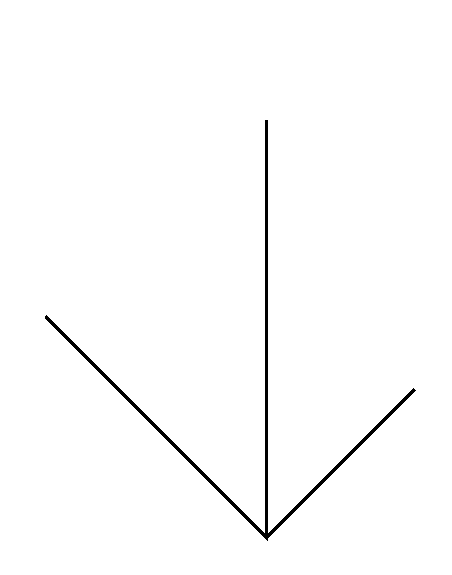
\includegraphics[width=5cm]{threeAngles}}{Mouvement par les  angles (3)}\label{xp:angle3}
	| pica berthe | 
	pica := Bot new. 
	\textbf{pica north.}
	pica jump: 200. 
	pica turnLeft: 180. 
	pica go: 200. 
	pica turnLeft: 180. 
	pica color: Color blue. 
	pica turnLeft: 45. 
	pica go: 150. 
	berthe := Bot new. 
	berthe north. 
	berthe color: Color red. 
	berthe turnRight: 45. 
	berthe go: 100. 
\end{scriptfigwithsize}


\begin{exonofigtitle}{Le Changement de Direction de R\'ef\'erence}
Continuons \`a nous exercer avec le Script ~\ref{xp:angle3} en changeant la direction de r\'ef\'erence. Par comparaison 
pour \^etre significatif, vous orientez\ct{berthe} dans la m\^eme direction que \ct{pica} apr\`es les avoir cr\'e\'es. Essayez 
les valeurs d'angles qu vous souhaitez et essayez de deviner quel dessin il en r\'esultera apr\`es l'ex\'ecution du script. 
Continuez de vous exercez avec ce script jusqu'\`a ce que vos pr\'edictions soient corrects.
\end{exonofigtitle}

Notons que vous devriez toujours \^etre capable de pr\'edire ce qui va ce passer avant d'avoir ex\'ecuter un script, 
parce qu'un ordinateur ex\'ecute aveugl\'ement toutes les d\'eclarations valides, m\^eme les plus stupides.

\section{Un Robot Horloge}

J'ai mentionn\'e que les lignes dessin\'ees dans le Script 4-6 sont voisines des aguilles d'une horloges. 
L'analogie entre le temps et les angles est bonne, la notion de degr\'es est fortement corr\'el\'ee avec celle 
des heures. Les anciennes civilisations ont d\'ecouvert la notion de temps en mesurant l'angle du soleil 
(ou des \'etoiles) par rapport \`a une direction de r\'ef\'erence. Toutefois, un script comme le Script 4-6 vous permet 
de placer les aiguilles dans une position qui n'indique pas un moment r\'eel de la journ\'ee. Par exemple, 
vous pouvez dessiner une horloge avec l'aiguille des heures pointant le nord et l'aiguille des minutes 
pointant le sud. Mais sur une vrai horloge, lorsque l'aiguille des minutes pointe le sud, c'est une demi heure, 
et donc l'aiguille des heures devra \^etre \`a mi-chemin entre deux nombres sur l'horloge.

Maintenant vous \'etudierez la relation entre l'aiguille des heures et des minutes sur une vrai horloge 
qui repr\'esente une heure r\'eelle de la journ\'ee.

%xp

\begin{exonofigtitle}{Une "Vrai" Horloge}
	Modifions le Script~\ref{xp:angle3} comme suit : 

\begin{itemize} 
	\item Gardez la direction de r\'ef\'erence au nord (comme pour le Script 4-6). Cette ligne de r\'ef\'erence 
	indique 12:00 midi ou minuit. 
	\item  Utilisez la m\'ethode \ct{turnRight:} pour les deux robots. Apr\`es tout, les aiguilles d'une horloge bouge 
	dans le sens des aiguilles d'une montre, qui est \`a droite.
	\item Vous pouvez demander \`a \ct{pica} de dessiner l'aiguille des minutes en multipliant le nombre de minutes 
	apr\`es l'heure que vous souhaiter indiquer par 6 (pendant les 60 minutes dans une heure, l'aiguille des minutes 
	traverse 6*60=360 degr\'es donc un cercle complet). Par exemple, pour repr\'esenter l'aiguilles des minutes \`a 
	20 minutes pour une certaine heure, vous devrez utiliser l'expression \ct{turnRight: 120} ($120 = 6  * 20$). 
	\item Vous pouvez demander \`a \ct{berthe} de dessiner l'aiguille des heures en multipliant le nombre d'heure 
	que vous souhaiter indiquer en pultipliant par 30 (12 heures pour 30 degr\'es par heure \'equivaut \`a 360 degr\'es) 
	et ajouter ensuite un-demi (0.5) degr\'e pour chaque minute pass\'e apr\`es l'heure, pour 60 minutes, l'aiguille des 
	heures bouge de 30 degr\'es. Par exemple, l'aiguille des heure est positionn\'e \`a 2heures avec le message \ct{turnRight: 60} 
	$(60 = 30 * 2)$, tandis que l'heure 4:26 exige que l'aiguille des heures soit positionn\'ee avec le message \ct{turnRight: 133} 
	$(133 = 30 * 4 + 26 * 0.5)$. 
\end{itemize}
Essayez d'indiquer quelques heures que vous choisirez avec ce script modifi\'e.
\end{exonofigtitle}
	
\section{Simples Dessins}

Pour commencer, nous avons ici un script qui dessine un triangle avec trois cot\'es \'egaux :


\begin{scriptfigwithsize}[0.4]{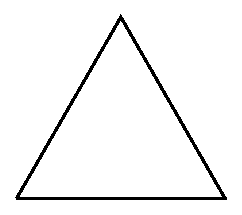
\includegraphics[width=3cm]{ChTurnfirstTriangle}}{Un Triangle Equilat\'eral}\label{xp:triangle}
	| pica | 
	pica := Bot new. 
	pica go: 100. 
	pica turnLeft: 120. 
	pica go: 100. 
	pica turnLeft: 120. 
	pica go: 100. 
	pica turnLeft: 120. 
\end{scriptfigwithsize}

La derni\`ere ligne du code n'est pas n'est pas n\'ecessaire pour dessiner le triangle, elle sert \`a refaire pointer 
\ct{pica} dans sa position initiale.

Maintenant, vous \^etes pr\^et \`a dessiner une maison. 

\begin{exofigwithsize}[0.5]{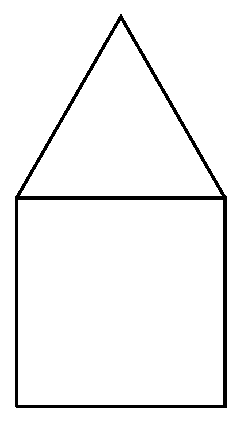
\includegraphics[width=2cm]{ChTurnbabyHouse}}{Une Maison}\label{xp:house}
	Dessinez une maison comme le montre la figure. Essayez de dessiner des maisons de formes diff\'erentes.
\end{exofigwithsize}


\section{Polygones R\'eguliers}

Un polygone r\'egulier est une figure compos\'ee de segments tous de m\^emes longueurs et qui ont des angles \'equivalents. 
Un triangle \'equilat\'eral est un polygone r\'egulier avec trois cot\'es. Un carr\'e est un polygone r\'egulier avec 
quatre cot\'es. Par exemple, le  Script~\ref{xp:triangle} dessine un triangle \'equilat\'eral qui a ses longueurs pour 
les cot\'es de 100 pixels. Il est obtenu en disant \`a \ct{pica} d'avancer de 100 pixels et ensuite de tourner 
de 120 degr\'es \`a gauche, et ensuite en r\'ep\'etant ces deux messages encore deux fois pour qu'il soit ex\'ecuter 
au total trois fois.

Vous pouvez programmer un robot pour dessiner un polygone r\'egulier avec un certain nombre de cot\'es en lui demandant 
de bouger d'une certaine longueur et ensuite de tourner \`a gauche ou \`a droite de 360 degr\'es divis\'es par le nombre de 
cot\'es ; cette s\'equence doit \^etre r\'ep\'et\'e autant de fois qu'il y a de cot\'es. Notons que la derni\`ere rotation du robot 
peut \^etre omis, du fait que le robot aura d\'ej\`a dessin\'e la derni\`ere ligne du polygone.


\begin{exofigwithsize}[0.5]{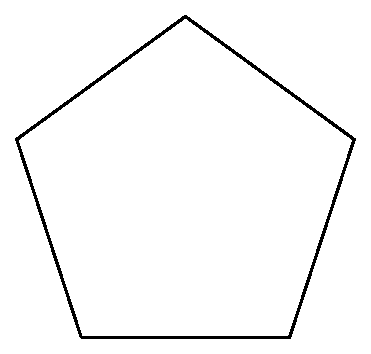
\includegraphics[width=2cm]{ChTurnpentagon}}{}\label{xp:penta}
	Dessinez un pentagone r\'egulier (un polygone r\'egulier \`a cinq cot\'es), comme le montre la figure, 
	avec des cot\'es de longueur 100 pixels.
\end{exofigwithsize}

\begin{exofigwithsize}[0.5]{\includegraphics[width=2cm]{ChTurnhexagon}}{}\label{xp:hexagon}
	Dessinez un hexagone r\'egulier (un polygone r\'egulier \`a six cot\'es), comme le montre la figure, avec des cot\'es de longueur 100 pixels.
\end{exofigwithsize}

Si vous \^etes curieux de voir jusqu'où vous pouvez aller avec ce proc\'ed\'e, vous pouvez utiliser la fonction 
copier et coller de l'espace de travail en g\'en\'erant un polygone r\'egulier avec un grand nombre de cot\'es. 
Si vous en avez envie, faite le en augmentant le nombre de cot\'es. Cependant, dans le Chapitre 7, je vous 
montrerai comment vous pouvez taper une s\'equence d'expressions et ensuite la r\'ep\'eter encore et encore.

\begin{exofigwithsize}[0.5]{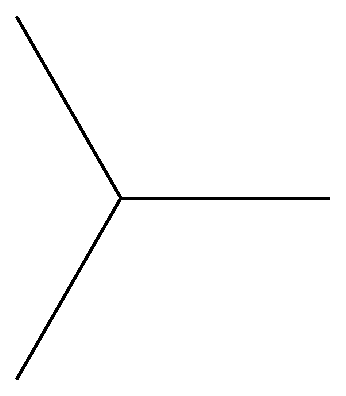
\includegraphics[width=2cm]{ChTurnc3pace}}{3 espaces}\label{xp:threespokedfig}
Dessinez les trois rayons comme le montre la figure ci-dessous. 
\end{exofigwithsize}


\section{R\'esum\'e}

\begin{itemize}
\item Un robot peut \^etre orient\'e relativement \`a sa direction courante en utilisant les m\'ethodes \ct{turnLeft}: 
et \ct{turnRight:}. 
\item Les param\`etres donn\'es pour les m\'ethodes \ct{turnLeft:} et \ct{turnRight:} sont donn\'es en degr\'es. 
\item Tourner de 360 degr\'es correspond \`a une rotation d'un cercle complet.
\item Tourner de 180 degr\'es correspond \`a une rotation d'un demi cercle. 
\item Les valeurs des angles qui diff\`erent par un multiple de 360 degr\'es sont \'equivalentes.
\end{itemize}

Ci-dessous, une liste des m\'ethodes que vous avez apprises tout au long de ce chapitre. 


\vspace*{5mm}
\noindent
\setlength{\extrarowheight}{1mm}
{\small \begin{tabular}{p{14mm}p{23mm}p{45mm}p{22mm}}
\hline
\textbf{M\'ethode} & \textbf{Syntaxe} & \textbf{Description} & \textbf{Exemple}\\
\hline
\textsf{turnLeft:} & \textsf{turnLeft: aNumber} &
Dit au robot de changer sa direction \`a gauche par un nombre donn\'e de degr\'es.
& \textsf{pica turnLeft: 30 } \\

\textsf{turnRight:} & \textsf{turnRight: aNumber} &
Dit au robot de changer sa direction \`a droite par un nombre donn\'e de degr\'es.
& \textsf{pica turnRight: 30} \\


\textsf{turn:} & \textsf{turn: aNumber} &
Dit au robot de changer sa direction par un nombre donn\'e de degr\'es en 
suivant la convention math\'ematique qu'une rotation est \`a gauche si le 
nombre est positif et \`a droite si il est n\'egatif.
& \textsf{pica turn: 30} \\

\textsf{beInvisible} & \textsf{beInvisible} &
Cache le r\'ecepteur. 
& \textsf{pica beInvisible} \\

\textsf{beVisible} & \textsf{beVisible} &
Montre le r\'ecepteur. 
& \textsf{pica beVisible} \\
\hline
\end{tabular}}


\ifx\wholebook\relax\else
    \end{document}
\fi


%%% Local Variables:
%%% coding: utf-8
%%% mode: latex
%%% TeX-master: t
%%% TeX-PDF-mode: t
%%% ispell-local-dictionary: "english"
%%% End:
